\section{How is the Development Affected by the Technical Possibilities?}\label{rq1}

Some of the wished development were too complex to be implemented during the master thesis. Below, it is described what future work is wished in the area.

\subsection{Data Analysis Improvements}
Today, data analysis of quiz results takes a tremendous amount of time, and new results are thus not instantly accessible to the stakeholders. The data needs to be acquired into Google Sheets, and then needs to be enhanced in several ways to be filterable and visualized, see section \ref{dataanalysisframework}. The raw data when inserted into Google Sheets can be seen in figure \ref{fig:unprocessedData}.

\begin{figure}[h]
  \centering
  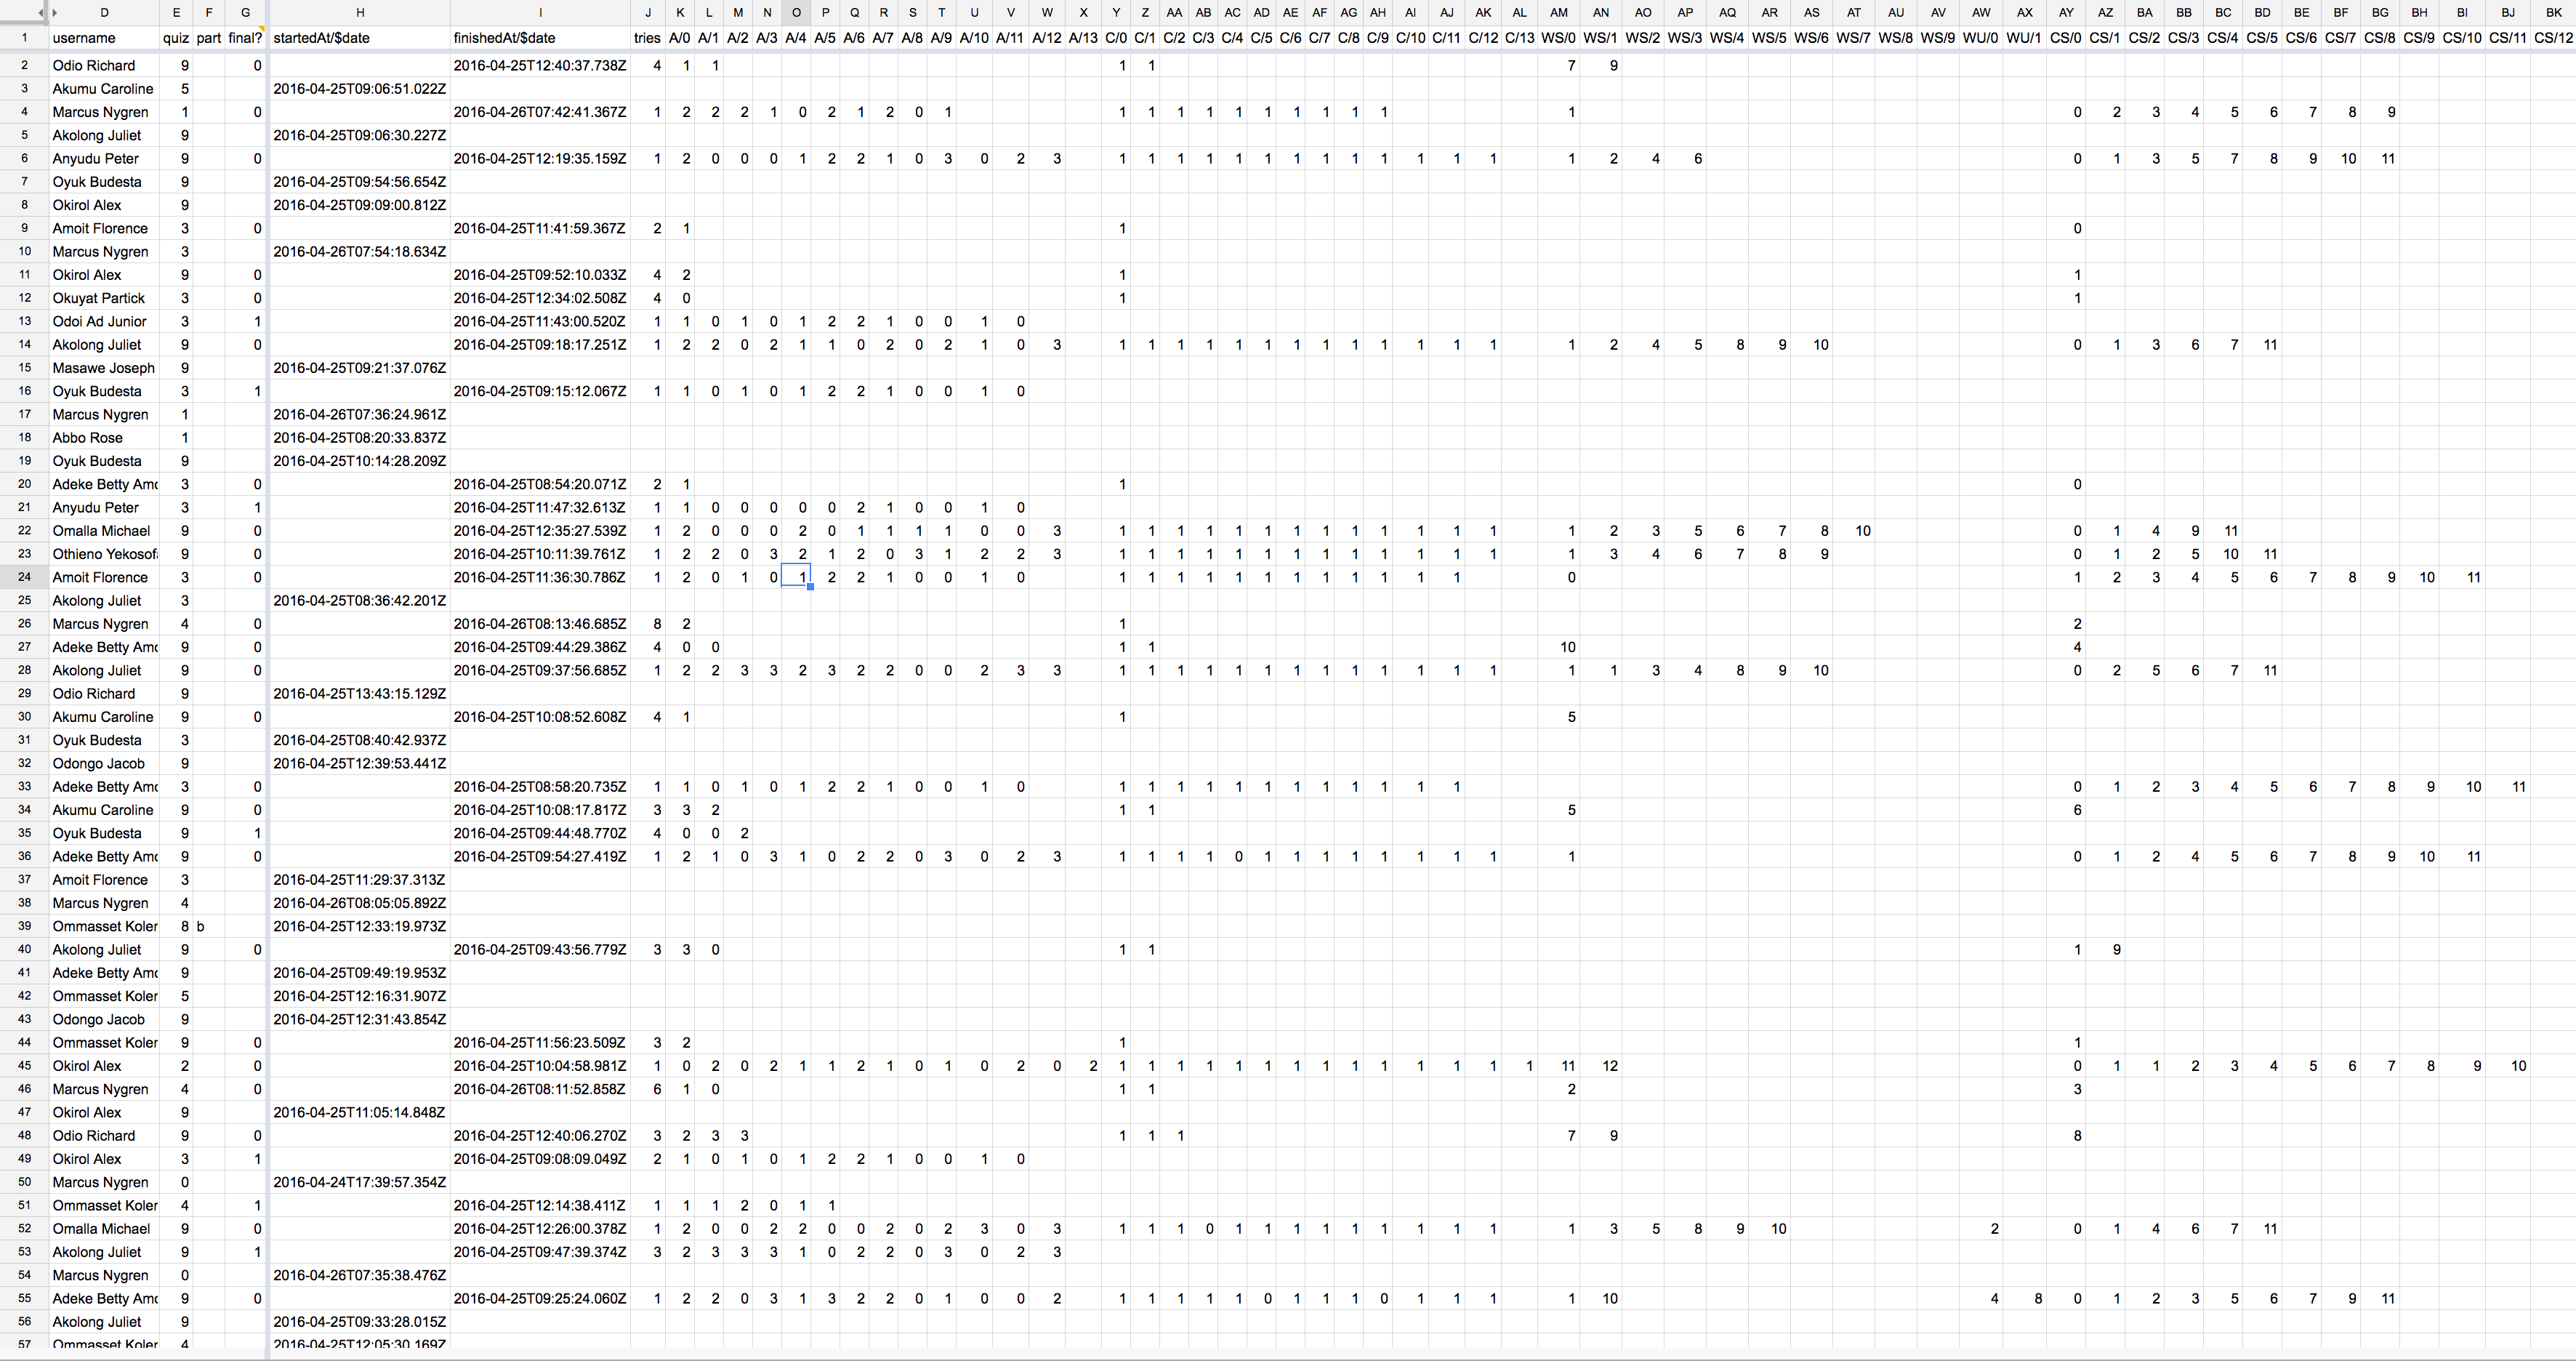
\includegraphics[width=0.8\textwidth]{analysis/unprocessedData.png}
  \caption{The raw data of the quiz results when inserted into Google Sheets. The purpose of the image is to explain how much work that is needed in order to process the data into insights.}
  \label{fig:unprocessedData}
\end{figure}

A lot of future development time should be spent so that most of this work is made automatically. Some of this work, is related to the way that the data is saved. Today, whether the coach was correct or incorrect on a question, and how many coaches answered that question incorrect after the first try, needs to be done by process of elimination, because the data is not properly structured in the database.

There were also a small number of errors with quiz submissions in iteration 4. Most notably, certification tests for coach quiz 9 were not submitted, which is why the paper submissions proved very valuable as a backup. To discover more errors regarding offline-online functionality, is important, as it is cumbersome and time-costly to test these manually. A good way to discover such errors, would be automatic tests (or regression tests), so that the app can be used by the coaches with confidence, without extra personnel present, checking that the app works.

\subsection{Code Quality}
Since the app will be continually used and developed by others in the future, code quality is important. React.js makes it easy to structure the code in a way that gives a new developer a good overview of the different components, and its functionality. Even so, refactoring the code into smaller components would be a good idea.

To increase speed of the app, refactoring the code to ensure that loading of assets happen more effectively (especially quiz questions), and also that data is cached in a logical way (saving necessary information so that it does not need to load the same information again, and vice versa), would be helpful. As the YoungDrive program grows and more people will use the app, there will be a lower tolerance for the app being slow. The app, especially on native, takes a long time to load, mostly because of asset loading.

\subsection{Availability in More Countries}\label{sec:internationalization}
During the Zambia tests, the coaches were given a Zambia version of the app, and in Uganda, they were given a Uganda version. In the future, it would be advisable if the coach ID used for login would affect if the Zambia version or the Uganda version should be shown.

As long as the users of the app, such as the coaches in Uganda and Zambia, does have sufficient English skills, it is acceptable that the app is solely in one language. As more countries are introduced, the app should be available in different languages.

A challenge today is that the Zambia uses a newer manual, and e.g. the national currency is different than Uganda's. That Zambia has updated manuals, means that some questions are new, some are removed, and some are re-formulated. But the teacher still wants to be able to compare quiz results between the different countries. Today, the quizzes were simply replaced between versions. This has the advantage of being easy to implement, but the clear disadvantage that the teacher can not compare quiz results between countries.

A good solution to internationalization of quizzes would be that each question in the database should include an unique ID, with different texts depending on country and coach manual. This would allow the teacher to keep track of some coaches have difficulties with a question, regardless of location.

\subsection{Availability on All Android Devices}
Since the introduction of Meteor 1.3, older Android devices are no longer supported. For the YoungDrive coaches, this is an issue, as most often devices use older Android operating systems, and does not have great performance. Today, a Meteor 1.2 version of the app is available on the AppStore. Also, the newest version is available on the web. However, in the future research should be put into if the app should abandon Meteor 1.3 altogether, or if there is another way to ensure backwards capability.

\subsection{Availability on Feature Phones}
As far from all coaches does not currently possess smartphones, few coaches will currently be able to use the developed app for preparing their youth sessions. Therefore, what was discovered in iteration 1, that all coaches possess feature phones, could guide the development of a SMS-based service. While this was not viable for the scope of the master thesis, research has been made into related work. A recommendation is to try VOTO Mobile \citep{voto-mobile}, which supports multiple-choice questions and internationalization. Today, this solution has been used mostly for doing evaluations in rural areas, via automatic phone calls where the caller can be given responses in text. However, research on using such a solution for educational purposes seems promising.

\subsection{Reaching Statistical Significance}
There are multiple examples how data analysis on a larger data sample could benefit. More than YoungDrive being able to take more informed choices regarding the future development of the app, it would strengthen answering the research questions. One such example is "Is the coach learning?". With enough data, it would be interesting to analyse the impact of feedback on getting the correct answer the next time. For example, you could compare if getting feedback on being wrong and unsure leads to better results than getting feedback on being wrong and unsure.
